\label{app:intuition}
\section{Additional Intuitions and Explainations}
\subsection{Extension to transformer backbone}
\label{app:transformer}
While this paper focuses on a causal implementation of \algo{} with RNNs, it's easy to adopt \algo{} with modern architectures like transformers. One can simply modify a transformer-based sequence diffusion model to train with independent noise levels across tokens and follow the techniques listed in Section \ref{app:snr_derivation}. A strict implementation of causal \algo{} would involve a causal attention mask on the transformer. However, \algo's fractional masking can do something more interesting: Consider the scenario that we use a transformer without a causal mask. We can still implement causality by controlling noise. By labeling the future as full white noise, there is no information leaked into the past tokens. By labeling future tokens as free of noise, we make the model completely non-causal. By labeling the future tokens as noisy, a slight amount of information about the future is provided for the prediction of past tokens. This effectively states that one only needs a non-causal architecture, but controlling fractional noise of the future, to achieve partial or complete causality. These extensions are beyond the scope of this paper, but we already verified their effectiveness and thus provide them as intuitions for future works.

\subsection{The need for independent noise levels}
\label{app:independent_noise}
When training \algo{}, we choose to sample per-token noise level following i.i.d uniform distribution from $[1,2...K]$. One may wonder about the necessity of this choice. Here we discuss the unique abilities of independent noise and the compute overhead added by it. 

The use of independent noise confers a number of special capabilities in our model, including stabilization of autoregressive rollout~\ref{par:stabilizing_autoreg}, modeling causal uncertainty~\ref{par:zigzag}, and removing the need for expensive reconstruction guidance when conditioning on context~\ref{app:cond_replacement}. None of these capabilities can be achieved by full-sequence diffusion. AR-diffusion~\cite{wu2023ar} and Rolling Diffusion~\cite{ruhe2024rolling} can only achieve the first and third one. There are more sampling-time applications such as flexible frame interpolation. Finally, we also saw the practical benefits of using independent noise in hyperparameter tuning. One can simply try different sampling schemes to figure out the most effective one for their applications. All these capabilities only require training the model once with \algo{}. In contrast, any tuning of the sampling scheme would require re-training the model for AR-diffusion and Rolling Diffusion.  

On the other hand, we didn't observe much computing overhead when comparing \algo{} to full-sequence diffusion, as soon as one closely follows our training techniques like~\ref{app:snr_derivation}. The empirical evidence is based on our experiments with an experimental transformer implementation of \algo{} and is thus not fully consistent with the main paper. However, we present the high-level descriptions below for readers interested in more insights: The complexity added by independent noise levels is in the temporal dimension. Therefore, we first adopt a standard technique for video diffusion models - image pre-training, to abstract away the complexity of the image pixels themselves. Then the complexity left is temporal prediction only. We then take the pre-trained image-only model and continue training it on video data. It turns out the sampling result of \algo{} with fewer training steps in this second stage is already better than that of full-sequence diffusion at convergence. We speculate that the better result is due to the same data-augmentation effect described in prior works~\cite{kingma2024understanding}. This shows that the overhead added by independent noise is well-warranted when considering the overall training compute (including image pre-training). 


\subsection{Guidance as planning}
\label{app:reward_guidance}
As stated in Section~\ref{sec:related_prelim}, one can use the gradient of the logarithmic of a classifier $\log c(y|\bx_t^k)$ to guide the sampling process of diffusion model towards samples with a desired attribute $y$. For example, $y$ can refer to the indicator of a success event.  However, we can consider the logarithmic of a more general \emph{energy function} $c(\bx_t^k)$. This has the interpretation as $\Pr(y | \bx_t^k)$, where $\Pr[ y= 1 \mid \bx_t^k] = e^{c(\bx_t^k)}$. Some popular candidate energies include
\begin{align}
    c(\bx_t^k) =\Exp\left[\sum_{t' > t} \br_{'}(\bx_{t'}^{k_{t'}}) \mid \bx_t^{k}\right],  \label{eq:cost_to_go_guidance}
\end{align}
corresponding to a cost-to-go; we can obtain unbiased estimates of this gradient by using cumulative reward $\tilde  c(\bx_t^k) =\sum_{t' > t} \br_{'}(\bx_{t'}^{k_{t'}})$. We can also use goal distance $c = - \|\bx_T^{k_T} - \mathbf{g}\|^2$ as a terminal reward. We provide details about the guidance function deployed in the maze2d planning experiment in Appendix~\ref{app:maze_guidance}.



\subsection{Noising and stabilizing long-horizon generations}\label{app:noising_long_horizons}
\newcommand{\ksmall}{k_{\mathrm{small}}}
Here, we explain in detail how we use noising to stabilize long-horizon generation. At each time $t$, during the denoising, we maintain a latent $\bz_{t-1}^{\ksmall}$ from the previous time step, with $0 < \ksmall \ll K$ corresponding to some small amount of noise. We then do \emph{next token} diffusion to diffuse the token $\bx_t$ across noise levels $\bx_t^{K},\bx_{t}^{K-1},\dots,\bx_t^0$ (corresponding to \Cref{alg:diffusion_forcing_sampling} with horizon $T = 1$, initial latent $\bz_{t-1}^k$, and noise schedule $\cK_{m,1} = m$); this process also produces latents $\bz_t^K,\bz_t^{K-1},\dots,\bz_t^0$ associated with each noise level. From these, we use the latent $\bz_t^{\ksmall}$ to repeat the process. This noised latent can be interpreted as an implementation of conditioning on $\bx_t^{\ksmall}$ in an autoregressive process. In a potential transformer implementation of \algo{} as we discussed in Appendix~\ref{app:transformer}, one can instead run a forward diffusion on a fully diffused token to achieve stabilization. 

It is widely appreciated that adding noise to data ameliorates long-term compounding error in behavior cloning applications \cite{ke2021grasping,laskey2017dart}, and even induces robustness to non-sequential adversarial attacks \cite{cohen2019certified}. In autoregressive video generation, the noised  $\bx_t^{\ksmall}$ is in-distribution for training, because \algo{} trains from noisy past observation in its training objective.
Hence, this method can be interpreted as a special case of the DART algorithm for behavior cloning \cite{laskey2017dart}, where the imitiator (in our case, video generator) is given actions (in our case, next video frames) from noisy observations (in our case, noised previous frames). Somewhat more precisely, because we use both tokens at training time to train \algo, and using slightly noised tokens for autoregression at test time, our approach inherits the theoretical guarantee of the HINT algorithm \cite{block2023provable}.



\subsection{Why Monte Carlo Guidance relies on \algo}
\label{app:cannot_mcg}
Monte Carlo Guidance provides substantial variance reduction in our estimate of cost-to-go guidance \eqref{eq:cost_to_go_guidance}. This technique crucially relies on the ability to roll out future tokens from current ones to use these sample rollouts to get Monte Carlo estimates for gradients. This is not feasible with full-sequence diffusion, because this requires denoising all tokens in tandem; thus, for a given fixed noise level, there is no obvious source of randomness to use for the Monte Carlo estimate. It may be possible to achieve variable horizon via the trick proposed in the following subsection to simulate future rollouts, but to our knowledge, this approach is nonstandard.  



\subsection{Does the replacement technique lead to flexible horizons in full-sequence diffusion?}
\label{app:cond_replacement}
A naive way to obtain flexible horizon generation in full-sequence diffusion is via the ``replacement trick'': consider a full sequence model trained to diffuse $\bx_{1:T}$, which we partition into $\bx_{1:t-1},\bx_{t:T}]$. Having diffused tokens $\bx_{1:t-1}$, we can attempt to denoise tokens of the form $[\tilde \bx_{1:t-1}^{k},\bx_{t:T}^k]$, where we \emph{fix} $\tilde \bx_{1:t-1}^{k} = \bx_{1:t-1}$ to be the previously generated token, and only have score gradients update the remaining $\bx_{t:T}^k$.  One clear disadvantage of this method is inefficiency - one still needs to diffuse the whole sequence even when there is one step left at $t=T-1$. What's more, \cite{ho2022video} points out that this approach of conditioning, named ``conditioning by replacement'', is both mathematically unprincipled and can lead to inconsistency in the generated sequence. The best fix proposed by~\cite{ho2022video} incorporates an additional gradient term with respect to $\bx_{t:T}$ at every diffusion step; this is still an incomplete fix and suffers the computation cost of an extra backward propagation for every sampling step.

\subsection{Further connection to Bayesian filtering}
The core idea of \algo{} can be interpreted as using diffusion to construct an interpolation between prior distribution and posterior distribution of a Bayes filter. Consider the hybrid distribution $p(\bz_t|\bz_{t-1}, \bx_t^k)$. When $k=0$, this hybrid distribution becomes the posterior $p(\bz_t|\bz_{t-1}, \bx_t)$. On the other hand, when $k=K$, the hybrid distribution becomes $p(\bz_t|\bz_{t-1}, \mathbf{n})$ for $ \mathbf{n}\sim \mathcal{N}(0, \mathbf{I})$. Since the independent Gaussian noise term $ \mathbf{n}$ contains no information about $ \bz$, this is exactly the prior distribution $p(\bz_t|\bz_{t-1})$. By varying $k$ between $K$ and $0$, the same neural network can parameterize everything between prior and posterior.

\begin{figure}
    \centering
    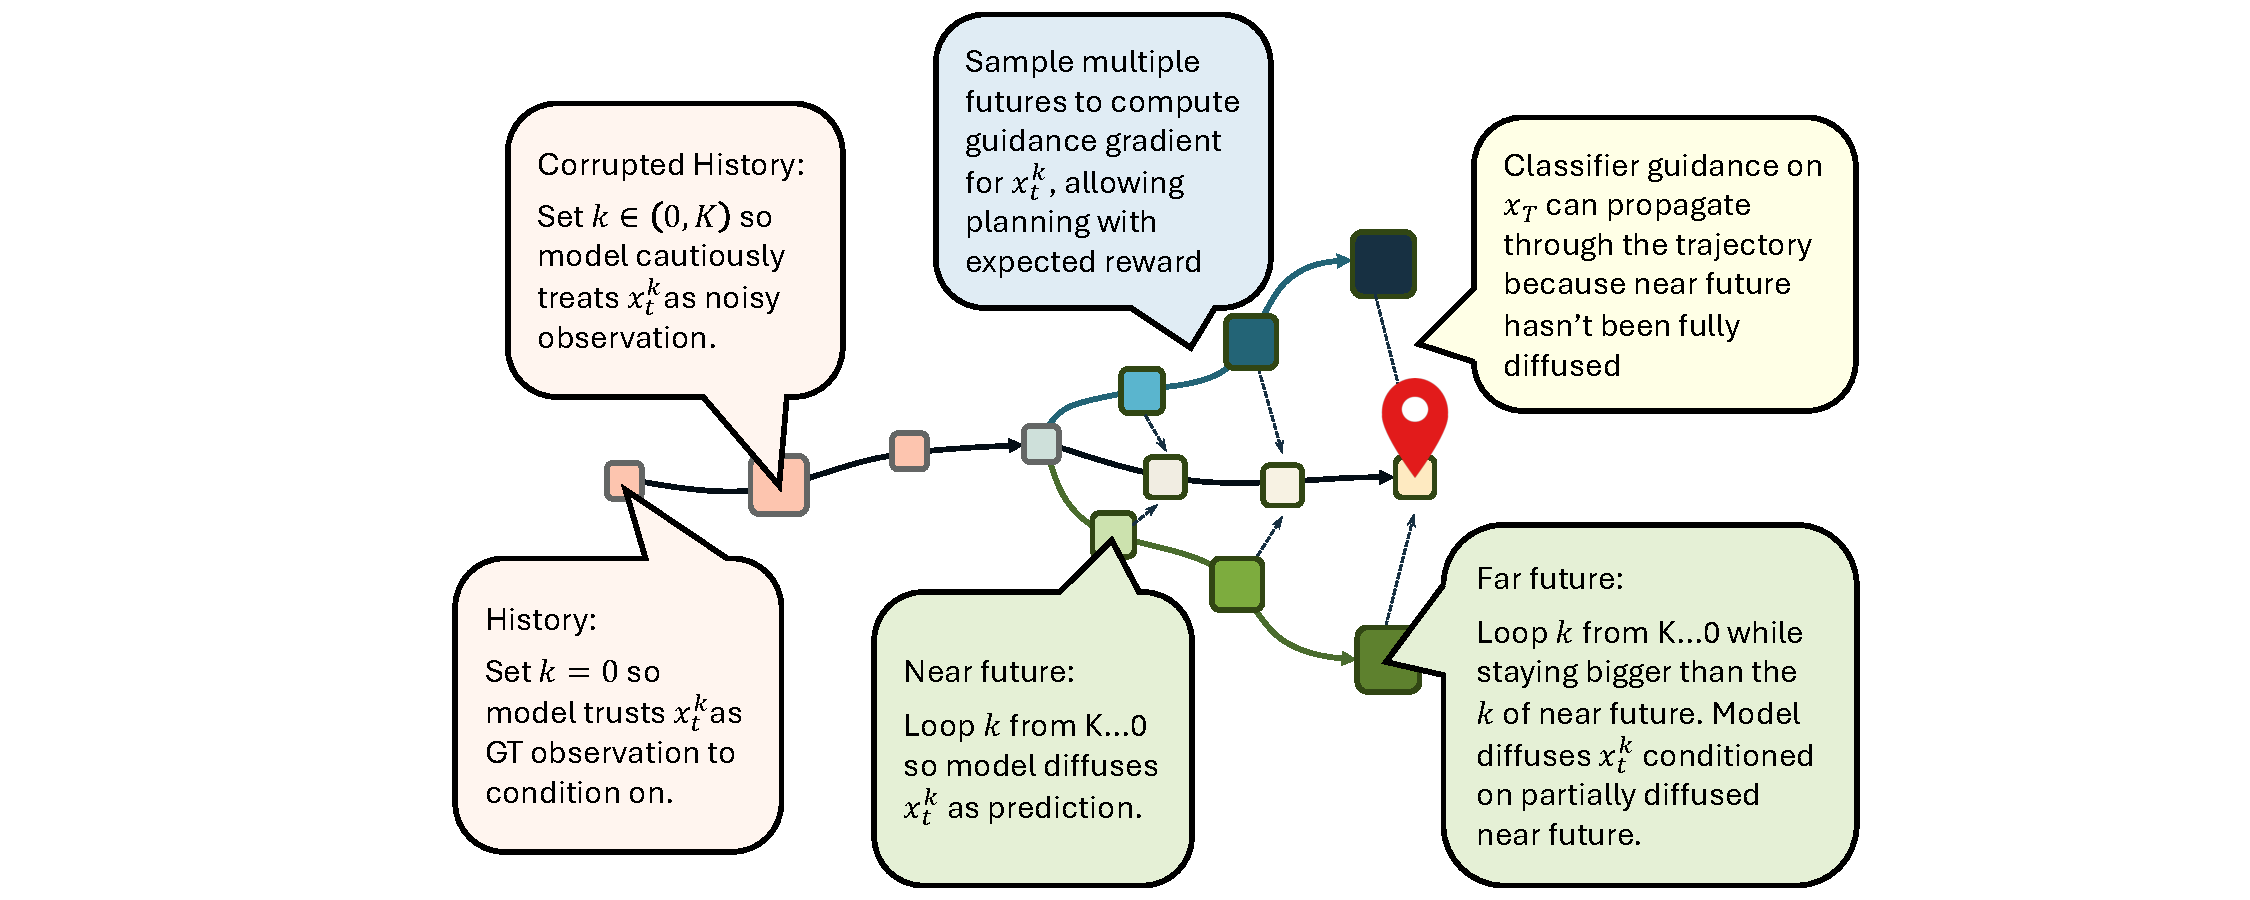
\includegraphics[width=0.8\textwidth]{figures/ability_in_sequence.pdf}
    \caption{\algo{} is trained on independent level of noises at different timesteps. As a result, we can control the noise level $k$ to achieve different effects on conditioning and prediction.}
    \label{fig:ability_in_seq}
\end{figure}

\subsection{Connection to other sequence training schemes}
Noise as masking provides a unified view of different sequence training schemes. The following exposition uses a length $3$ sequence as an example: We always start with fully masked sequence $[\bx_1^K,\bx_2^K,\bx_3^K]$ with the goal of denoising it a ``clean sequence'' of zero noise. $[\bx_1^0,\bx_2^0,\bx_3^0]$. Assume all diffusions are sampled with $3$-step DDIM.

\paragraph{Autoregressive.} In teacher forcing, one trains a model to predict the next token conditioned on prior observations. One can train next-token diffusion models with teacher forcing such as ~\cite{rasul2021autoregressive}: feed neural network with past observations as well as a current observation and ask it to predict clean current observation. A typical training pair can have the input of $[\bx_1^0,\bx_2^0,\bx_3^{K}]^\top$ and target of $[\bx_1^0,\bx_2^0,\bx_3^{0}]^\top$.

At sampling time, one fully diffuses the next token before adding the diffused observation to history to perform an autoregressive rollout. The diffusion process would thus look like 
\begin{align*}
&[\bx_1^K,\bx_2^K,\bx_3^K]^\top\\
&[\bx_1^{K//2},\bx_2^K,\bx_3^K]^\top,\\
&[\bx_1^{0},\bx_2^{K},\bx_3^{K}]^\top,\\
&[\bx_1^{0},\bx_2^{K//2},\bx_3^{K}]^\top\\
&[\bx_1^{0},\bx_2^{0},\bx_3^{K}]^\top,\\
&[\bx_1^{0},\bx_2^{0},\bx_3^{K//2}]^\top,\\
&[\bx_1^{0},\bx_2^{0},\bx_3^{0}]^\top.
\end{align*}
Notably, \algo{} can also perform this sampling scheme at sampling time for applications like imitation learning, when one wants to diffuse the next action as fast as possible.

\paragraph{Full Sequence Diffusion.}
Full sequence diffusion models accept a noisy sequence and denoises level-by-level
\begin{align*}
&[\bx_1^K,\bx_2^K,\bx_3^K]^\top\\
&[\bx_1^{K//2},\bx_2^{K//2},\bx_3^{K//2}]^\top,\\
&[\bx_1^{0},\bx_2^{0},\bx_3^{0}]^\top.
\end{align*}
Notably, \algo{} can also perform this sampling scheme at sampling time.

\paragraph{Diffusion Forcing with causal uncertainty}
As shown in Figure~\ref{fig:method}, to model causal uncertainty, \algo{} keeps the far future more uncertain than the near future by having a larger noise level $k$, at any time of diffusion. An example pattern looks like this:
\begin{align*}
&[\bx_1^K,\bx_2^K,\bx_3^K]^\top\\
&[\bx_1^{K//2},\bx_2^K,\bx_3^K]^\top,\\
&[\bx_1^{0},\bx_2^{K//2},\bx_3^{K}]^\top,\\
&[\bx_1^{0},\bx_2^{0},\bx_3^{K//2}]^\top\\
&[\bx_1^{0},\bx_2^{0},\bx_3^{0}]^\top
\end{align*}
Notable, ~\cite{wu2023ardiffusion} is the first one to propose such a linear uncertainty sampling scheme for causal diffusion models, although \algo{} provides a generalization of such scheme in combination with other abilities.

\paragraph{Diffusion Forcing with stablization}
Previously we introduced the autoregressive sampling scheme that \algo{} can also do. However, such a scheme can accumulate single-step errors because it treats predicted $\bx$ as ground truth observation. \algo{} addresses this problem by telling the model that generated images should be treated as noisy ground truth, as shown in~\ref{fig:method}. 

It first fully diffuses the first token, 
\begin{align*}
&[\bx_1^K,\bx_2^K,\bx_3^K]^\top\\
&[\bx_1^{K//2},\bx_2^K,\bx_3^K]^\top,\\
&[\bx_1^{0},\bx_2^{K},\bx_3^{K}]^\top\\
\end{align*}
Then, it feed the diffused $\bx_1^0$ into the model but tell it is of a slightly higher noise level, as $\bx_1^{1}$ to diffuse $\bx_2$.
\begin{align*}
&[\bx_1^{1},\bx_2^{K//2},\bx_3^{K}]^\top\\
&[\bx_1^{1},\bx_2^{0},\bx_3^{K}]^\top
\end{align*}
Then, it feeds the diffused $\bx_2^0$ into the model but tells it is of a higher noise level, as $\bx_2^{1}$.
\begin{align*}
&[\bx_1^{1},\bx_2^{1},\bx_3^{K//2}]^\top,\\
&[\bx_1^{1},\bx_2^{1},\bx_3^{0}]^\top.
\end{align*}

